%
% Presentation example
% Tibault Reveyrand - http://www.microwave.fr
%
% http://www.microwave.fr/LaTeX.html
% ---------------------------------------


%%%%%%%%%%%%%%%%%%%%%%%%%%%%%%% beamer %%%%%%%%%%%%%%%%%%%%%%%%%%%%%%%%%%%%%%%%%%%%%%%%%
% To run - pdflatex filename.tex
%	   acroread filename.pdf
%%%%%%%%%%%%%%%%%%%%%%%%%%%%%%%%%%%%%%%%%%%%%%%%%%%%%%%%%%%%%%%%%%%%%%%%%%%%%%%%%%%%%%%%

%\documentclass[compress,brown]{beamer}
\documentclass[compress,brown,xcolor=table]{beamer}

\usepackage{etex}
\mode<presentation>

\usetheme{Warsaw} %Warsaw
% other themes: AnnArbor, Antibes, Bergen, Berkeley, Berlin, Boadilla, boxes, CambridgeUS, Copenhagen, Darmstadt, default, Dresden, Frankfurt, Goettingen,
% Hannover, Ilmenau, JuanLesPins, Luebeck, Madrid, Maloe, Marburg, Montpellier, PaloAlto, Pittsburg, Rochester, Singapore, Szeged, classic

%\usecolortheme{lily}
% color themes: albatross, beaver, beetle, crane, default, dolphin, dov, fly, lily, orchid, rose, seagull, seahorse, sidebartab, structure, whale, wolverine

%\usefonttheme{serif}
% font themes: default, professionalfonts, serif, structurebold, structureitalicserif, structuresmallcapsserif



\hypersetup{pdfpagemode=FullScreen} % makes your presentation go automatically to full screen

% define your own colors:
\definecolor{Red}{rgb}{1,0,0}
\definecolor{Blue}{rgb}{0,0,1}
\definecolor{Green}{rgb}{0,1,0}
\definecolor{magenta}{rgb}{1,0,.6}
\definecolor{lightblue}{rgb}{0,.5,1}
\definecolor{lightpurple}{rgb}{.6,.4,1}
\definecolor{gold}{rgb}{.6,.5,0}
\definecolor{orange}{rgb}{1,0.4,0}
\definecolor{hotpink}{rgb}{1,0,0.5}
\definecolor{newcolor2}{rgb}{.5,.3,.5}
\definecolor{newcolor}{rgb}{0,.3,1}
\definecolor{newcolor3}{rgb}{1,0,.35}
\definecolor{darkgreen1}{rgb}{0, .35, 0}
\definecolor{darkgreen}{rgb}{0, .6, 0}
\definecolor{darkred}{rgb}{.75,0,0}

\xdefinecolor{olive}{cmyk}{0.64,0,0.95,0.4}
\xdefinecolor{purpleish}{cmyk}{0.75,0.75,0,0}

% can also choose different themes for the "inside" and "outside"

% \usepackage{beamerinnertheme_______}
% inner themes include circles, default, inmargin, rectangles, rounded

% \usepackage{beamerouterthemesmoothbars}
% outer themes include default, infolines, miniframes, shadow, sidebar, smoothbars, smoothtree, split, tree

\useoutertheme[subsection=false]{smoothbars}

% to have the same footer on all slides
%\setbeamertemplate{footline}[text line]{STUFF HERE!}
\setbeamertemplate{footline}[text line]{} % makes the footer EMPTY

% include packages
\usepackage{subfigure}
\usepackage{multicol}
\usepackage{amsmath}
\usepackage{epsfig}
\usepackage{graphicx}
\usepackage[all,knot]{xy}
\xyoption{arc}
\usepackage{url}
\usepackage{multimedia}
\usepackage{hyperref}

\usepackage{tikz}

\usetikzlibrary{automata,positioning, babel}

% Package pour le français
\usepackage[utf8]{inputenc}
\usepackage[french]{babel} % Pour adopter les règles de typographie française
\usepackage[T1]{fontenc} % Pour que LaTeX comprenne les caractères accentués ;
                         % norme iso-8859, cela risque de ne pas marcher avec
                         % des fichiers créés sous windows


     
%%%%%%%%%%%%%%%
%%%%%%%%%%%%%%%%%%%%%%%%%%%%%% Title Page Info %%%%%%%%%%%%%%%%%%%%%%%%%%%%%%%%%%%%%%%%%%%%

\title{Definición e implementación de un protocolo de aplicación}
\author{Johanna Capote Robayna \\ Guillermo Galindo Ortuño}
\institute{Fudamentos de Redes}
\date{}
%%%%%%%%%%%%%%%
%%%%%%%%%%%%%%%%%%%%%%%%%%%%%% Begin Your Document %%%%%%%%%%%%%%%%%%%%%%%%%%%%%%%%%%%%%%%


\begin{document}

%%%%%%%%%%%%%%%

\frame{
	\titlepage 
}

%%%%%%%%%%%%%%%

%  \frame{\tableofcontents}

%%%%%%%%%%%%%%%

\section*{Introduction}


%%%%%%%%%%%%%%%
% INTRODUCTION
%%%%%%%%%%%%%%%

% =================================================================
\begin{frame}{Descripción de la aplicación}
	\begin{itemize}
		\item Cliente: Usuarios que quiren encriptar o desencriptar un texto
		\item Servidor: Encriptador/Desencriptador que atiende las peticiones
		\item Sockets TCP		
	\end{itemize}	
\end{frame}

\section*{Diagrama}
\begin{frame}{Diagrama de estados}
	$A=USER*PASS*TXT*$\quad \quad $B=USER*PASS*$ 
	\begin{figure}
		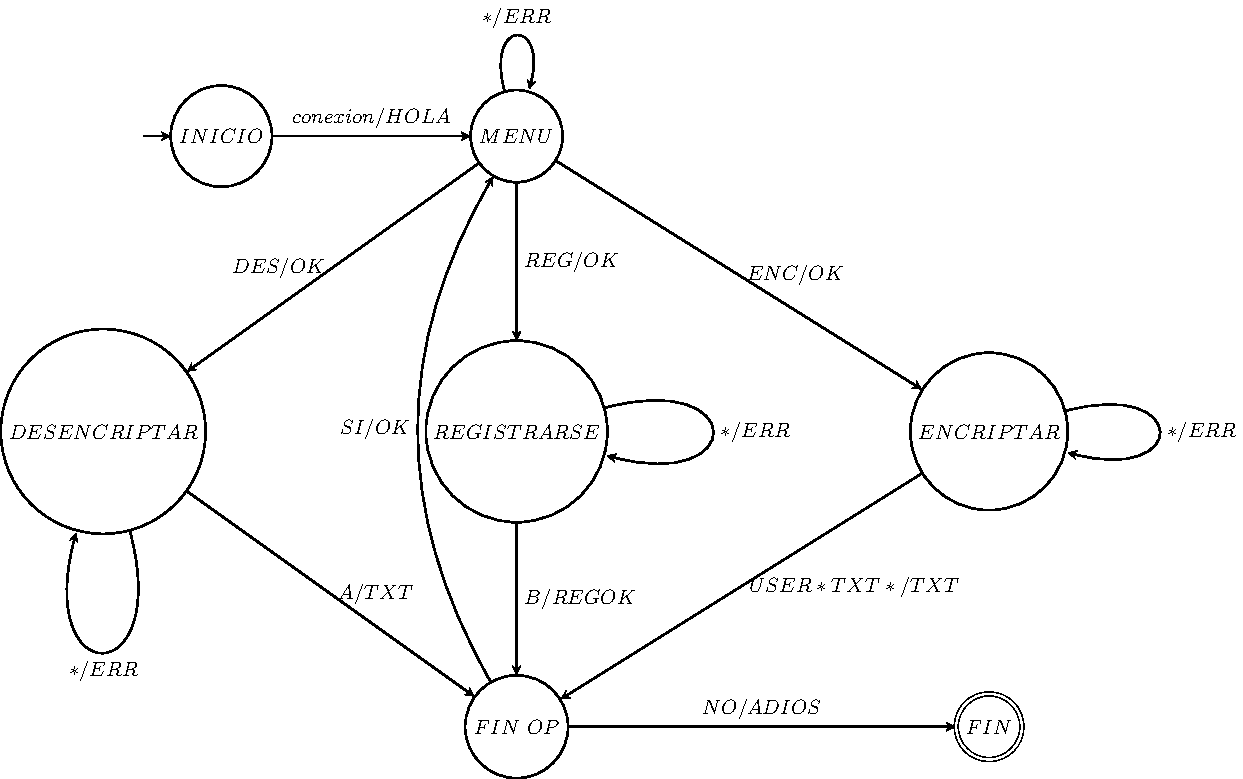
\includegraphics[width=10cm]{../pdf/diagrama.pdf}
		\centering		
		\label{p4}
	\end{figure}

\end{frame}

\section*{Mensajes}
\begin{frame}{Mensajes que intervienen}

\begin{table}[x]
\centering
\begin{tabular}{|l|l|l|}
\hline
\rowcolor[HTML]{963400} 
{\color[HTML]{FFFFFF} Código} & {\color[HTML]{FFFFFF} Cuerpo} & {\color[HTML]{FFFFFF} Descripción}                        \\ \hline
1001                          & HOLA                          & Conexión establecida correctamente                        \\ \hline
1002                          & DES                           & Petición de desencriptacion                                     \\ \hline
1003                          & ENC                           & Petición de encriptación                                       \\ \hline
1004                          & REG                           & Petición de registro                                      \\ \hline
1005                          & DES                           & Petición de desencriptar                                  \\ \hline
1006                          & OK                        	  & Opción escogida correcta                                      \\ \hline
1007                          & A                             & Mensaje con un texto a desencriptar y las\\  
							  & 							  & credenciales del receptor                                 \\ \hline
1008                          & TXT                           & Texto obtenido tras encriptar o \\
							  &                               &desencriptar \\ \hline
1009                          & B                         	  & Credenciales para registrarse                             \\ \hline
1010                          & REGOK                         & Registro exitoso                               \\ \hline
1011                          & $USER*TXT*$                   & Texto a encriptar y usario destino                            \\ \hline
1012                          & SI                            & Seguir realizando operaciones                                   \\ \hline
1013                          & ADIOS                         & Desconexión del programa                                  \\ \hline
\end{tabular}
\end{table}

\end{frame}

\end{document}

